\section*{Introduction}
Inference about epidemic dynamics commonly relies on observations such as confirmed cases, hospitalizations, and deaths to infer latent infection incidence \cite{irons2021estimating,miller2022statistical}. These observations are generated through biological progression, healthcare seeking, testing, and reporting, and therefore provide an incomplete and temporally distorted view of the underlying epidemic process \cite{eales2024key,greene2021nowcasting,costa2021covid}. The resulting observation process determines which temporal information about the underlying epidemic remains available for statistical inference (Fig.~\ref{fig:intro}A--F). Information about rapid temporal variation is preferentially attenuated during the observation process, making short-timescale epidemic dynamics progressively less distinguishable than slower variations (Fig.~\ref{fig:intro}D--H). Consequently, under a given delay and observation process, surveillance observations possess a finite temporal resolution beyond which distinct upstream epidemic trajectories become statistically indistinguishable, independent of the particular reconstruction algorithm employed. This raises a question that precedes reconstruction itself: which differences between epidemic histories are identifiable from the observations, and which remain underdetermined by the observations themselves?


\begin{figure*}[!t]
    \centering
    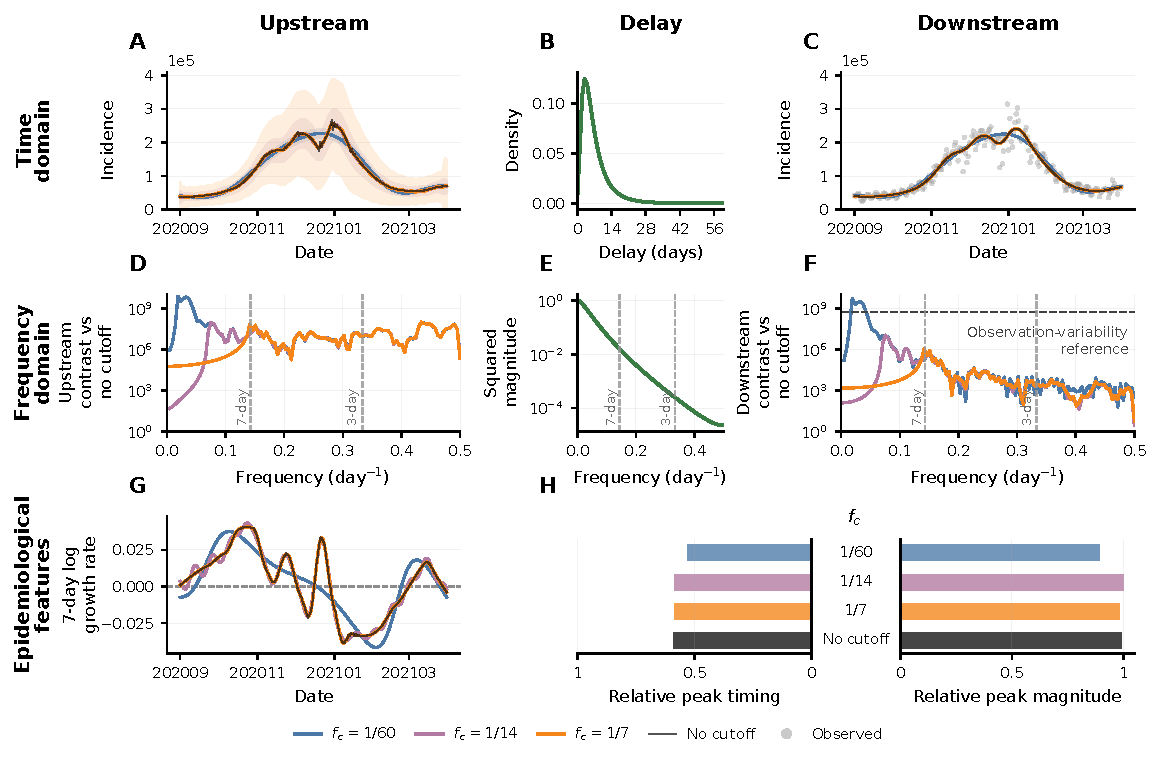
\includegraphics[width=\textwidth]{figs/epi_features_combined_us.pdf}
    \caption{
    \textbf{Delayed observations progressively reduce temporal information available for epidemic inference.}
    Columns show the upstream incidence scale, the delay process, and the downstream surveillance scale. Each colored upstream reference is constrained to Fourier components with \(f\leq f_c\).
    (\textit{A}) Frequency-constrained upstream reference trajectories estimated from U.S. confirmed-case incidence, with shaded bands showing locally non-identifiable perturbations.
    (\textit{B}) COVID-19 symptom-onset-to-report delay distribution \cite{zhang2020evolving}.
    (\textit{C}) Delay-convolved downstream reference trajectories and observed U.S. daily confirmed-case incidence \cite{dong2020interactive}.
    (\textit{D--F}) Upstream spectral contrast, squared delay-kernel magnitude, and downstream spectral contrast.
    (\textit{G,H}) Seven-day log growth rates and relative peak summaries derived from the same reference trajectories.
    Colors denote cutoff-specific references; black denotes the no-cutoff reference, and gray points denote observed incidence.
    Displayed spectra omit the zero-frequency component. Construction details are provided in Appendices~\ref{sec:Appendix_S2} and \ref{sec:Appendix_S3}.
    }
    \label{fig:intro}
\end{figure*}


Existing work has primarily addressed this question by developing methods to reconstruct latent epidemic trajectories from delayed observations, including back-projection\cite{becker1991method}, deconvolution\cite{goldstein2009reconstructing}, Bayesian latent-incidence reconstruction\cite{chitwood2022reconstructing}, and renewal-based inference\cite{cori2013new, gostic2020practical}. Reconstructing latent incidence from delayed observations remains an ill-posed inverse problem because multiple upstream trajectories may be consistent with the same downstream observations\cite{miller2022statistical}. Stable inference therefore requires regularization, prior distributions, or mechanistic constraints that select among multiple trajectories compatible with the observed data \cite{miller2022statistical, becker1991method, king2016statistical}. Posterior uncertainty quantifies what remains uncertain after introducing regularization and modeling assumptions, whereas observation-level identifiability asks what is determined by the observations themselves. This distinction motivates a broader question that extends beyond epidemic reconstruction itself.

Related concepts have also been developed in control theory and statistical detection theory. In control theory, observability characterizes whether latent states are recoverable from observations under specified dynamical and observation models\cite{kalman1960new,ljung1998system}. Statistical detection theory instead quantifies the distinguishability of competing signals or hypotheses in noisy observations using likelihood-based measures that underpin ideal-observer analyses in communication systems, signal processing, and medical imaging\cite{green1966signal,barrett2013foundations,barrett1998objective}. Neither framework directly characterizes the observation-level identifiability of epidemic trajectories under realistic delay distributions and observation noise. Addressing this gap requires linking epidemic delay processes and observation noise to likelihood-based measures of statistical distinguishability.

The epidemic observation process admits a natural spectral representation because convolution with a delay distribution becomes multiplication in the frequency domain\cite{oppenheim1999discrete,brigham1988fast}. This representation directly characterizes how temporal information is preserved across frequencies, with realistic epidemic delay distributions preferentially suppressing high-frequency components before they appear in downstream observations (Fig.~\ref{fig:intro}D–F)\cite{chitwood2022reconstructing,mcgough2020nowcasting}. Because statistical distinguishability depends on the information preserved by the observation process, observation-level identifiability is likewise expected to vary systematically across temporal scales. 

Motivated by this observation, we develop a general framework for characterizing observation-level identifiability based on a spectral representation of delayed epidemic observations. By combining the frequency response of epidemiologically realistic delay distributions with observation-model-specific likelihood weights, we derive a separability functional that determines whether differences between upstream trajectories remain recoverable in downstream surveillance data. This formulation yields explicit identifiability limits across common observation models and characterizes which temporal features are recoverable from the observations themselves, independent of the particular reconstruction method employed.
